% -*- coding: utf-8 -*-
%\documentclass[output=paper]{LSP/langsci} 
\documentclass[output=paper
,newtxmath
,modfonts
,nonflat]{langsci/langscibook} 
% \bibliography{localbibliography} 
% \usepackage{pifont}
\usepackage{savesym}

\savesymbol{downingtriple}
\savesymbol{downingdouble}
\savesymbol{downingquad}
\savesymbol{downingquint}
\savesymbol{suph}
\savesymbol{supj}
\savesymbol{supw}
\savesymbol{sups}
\savesymbol{ts}
\savesymbol{tS}
\savesymbol{devi}
\savesymbol{devu}
\savesymbol{devy}
\savesymbol{deva}
\savesymbol{N}
\savesymbol{Z}
\savesymbol{circled}
\savesymbol{sem}
\savesymbol{row}
\savesymbol{tipa}
\savesymbol{tableauxcounter}
\savesymbol{tabhead}
\savesymbol{inp}
\savesymbol{inpno}
\savesymbol{g}
\savesymbol{hanl}
\savesymbol{hanr}
\savesymbol{kuku}
\savesymbol{ip}
\savesymbol{lipm}
\savesymbol{ripm}
\savesymbol{lipn}
\savesymbol{ripn} 
% \usepackage{amsmath} 
% \usepackage{multicol}
\usepackage{qtree} 
\usepackage{tikz-qtree,tikz-qtree-compat}
% \usepackage{tikz}
\usepackage{upgreek}


%%%%%%%%%%%%%%%%%%%%%%%%%%%%%%%%%%%%%%%%%%%%%%%%%%%%
%%%                                              %%%
%%%           Examples                           %%%
%%%                                              %%%
%%%%%%%%%%%%%%%%%%%%%%%%%%%%%%%%%%%%%%%%%%%%%%%%%%%%
% remove the percentage signs in the following lines
% if your book makes use of linguistic examples
\usepackage{tipa}  
\usepackage{pstricks,pst-xkey,pst-asr}

%for sande et al
\usepackage{pst-jtree}
\usepackage{pst-node}
%\usepackage{savesym}


% \usepackage{subcaption}
\usepackage{multirow}  
\usepackage{./langsci/styles/langsci-optional} 
\usepackage{./langsci/styles/langsci-lgr} 
\usepackage{./langsci/styles/langsci-glyphs} 
\usepackage[normalem]{ulem}
%% if you want the source line of examples to be in italics, uncomment the following line
% \def\exfont{\it}
\usetikzlibrary{arrows.meta,topaths,trees}
\usepackage[linguistics]{forest}
\forestset{
	fairly nice empty nodes/.style={
		delay={where content={}{shape=coordinate,for parent={
					for children={anchor=north}}}{}}
}}
\usepackage{soul}
\usepackage{arydshln}
% \usepackage{subfloat}
\usepackage{langsci/styles/langsci-gb4e} 
   
% \usepackage{linguex}
\usepackage{vowel}

\usepackage{pifont}% http://ctan.org/pkg/pifont
\newcommand{\cmark}{\ding{51}}%
\newcommand{\xmark}{\ding{55}}%
 
 
 %Lamont
 \makeatletter
\g@addto@macro\@floatboxreset\centering
\makeatother

\usepackage{newfloat} 
\DeclareFloatingEnvironment[fileext=tbx,name=Tableau]{tableau}
% %% hyphenation points for line breaks
%% Normally, automatic hyphenation in LaTeX is very good
%% If a word is mis-hyphenated, add it to this file
%%
%% add information to TeX file before \begin{document} with:
%% %% hyphenation points for line breaks
%% Normally, automatic hyphenation in LaTeX is very good
%% If a word is mis-hyphenated, add it to this file
%%
%% add information to TeX file before \begin{document} with:
%% %% hyphenation points for line breaks
%% Normally, automatic hyphenation in LaTeX is very good
%% If a word is mis-hyphenated, add it to this file
%%
%% add information to TeX file before \begin{document} with:
%% \include{localhyphenation}
\hyphenation{
affri-ca-te
affri-ca-tes
com-ple-ments
par-a-digm
Sha-ron
Kings-ton
phe-nom-e-non
Daul-ton
Abu-ba-ka-ri
Ngo-nya-ni
Clem-ents 
King-ston
Tru-cken-brodt
Tab-leau
cophono-logies
mark-edness
Ti-gri-nya
a-mong
Car-stens
Lu-bu-ku-su
}
\hyphenation{
affri-ca-te
affri-ca-tes
com-ple-ments
par-a-digm
Sha-ron
Kings-ton
phe-nom-e-non
Daul-ton
Abu-ba-ka-ri
Ngo-nya-ni
Clem-ents 
King-ston
Tru-cken-brodt
Tab-leau
cophono-logies
mark-edness
Ti-gri-nya
a-mong
Car-stens
Lu-bu-ku-su
}
\hyphenation{
affri-ca-te
affri-ca-tes
com-ple-ments
par-a-digm
Sha-ron
Kings-ton
phe-nom-e-non
Daul-ton
Abu-ba-ka-ri
Ngo-nya-ni
Clem-ents 
King-ston
Tru-cken-brodt
Tab-leau
cophono-logies
mark-edness
Ti-gri-nya
a-mong
Car-stens
Lu-bu-ku-su
}
% %add all your local new commands to this file
\newcommand{\downingquad}[4]{\parbox{2.5cm}{#1}\parbox{3.5cm}{#2}\parbox{2.5cm}{#3}\parbox{3.5cm}{#4}}
\newcommand{\downingtriple}[3]{\parbox{4.5cm}{#1}\parbox{3cm}{#2}\parbox{3cm}{#3}}
\newcommand{\downingdouble}[2]{\parbox{4.5cm}{#1}\parbox{6cm}{#2}}
\newcommand{\downingquint}[5]{\parbox{1.75cm}{#1}\parbox{2.25cm}{#2}\parbox{2cm}{#3}\parbox{3cm}{#4}\parbox{2cm}{#5}}
\newcolumntype{Y}{>{\centering\arraybackslash}X}
\newcolumntype{T}{>{\centering\arraybackslash}m{2cm}}

%commands for Kusmer paper below
\newcommand{\ip}{$\upiota$}
\newcommand{\lipm}{(\_{\ip-Max}}
\newcommand{\ripm}{)\_{\ip-Max}}
\newcommand{\lipn}{(\_{\ip}}
\newcommand{\ripn}{)\_{\ip}}
\renewcommand{\_}[1]{\textsubscript{#1}}


%commands for Pillion paper below
\newcommand{\suph}{\textipa{\super h}}
\newcommand{\supj}{\textipa{\super j}}
\newcommand{\supw}{\textipa{\super w}}
\newcommand{\ts}{\textipa{\t{ts}}}
\newcommand{\tS}{\textipa{\t{tS}}}
\newcommand{\devi}{\textipa{\r*i}}
\newcommand{\devu}{\textipa{\r*u}}
\newcommand{\devy}{\textipa{\r*y}}
\newcommand{\deva}{\textipa{\r*a}}
\renewcommand{\N}{\textipa{N}}
\newcommand{\Z}{\textipa{Z}}
% 

%commands for Diercks paper below
\newcommand{\circled}[1]{\begin{tikzpicture}[baseline=(word.base)]
\node[draw, rounded corners, text height=8pt, text depth=2pt, inner sep=2pt, outer sep=0pt, use as bounding box] (word) {#1};
\end{tikzpicture}
}

%commands for Pesetsky paper below
% \newcommand{\sem}[2][]{\mbox{$[\![ $\textbf{#2}$ ]\!]^{#1}$}}
\newcommand{\sem}[2][]{\mbox{$[[ $\textbf{#2}$ ]]^{#1}$}}

% \newcommand{\ripn}{{\color{red}ripn}}%this is used but never defined. Please update the definition



%commands for Lamont paper below
\newcommand{\row}[4]{
	#1. & 
    /{#2}/ & 
    [{#3}] & 
    `#4' \\ 
}
%\newcounter{tableauxcounter}
\newcommand{\tabhead}[2]{
%     \captionsetup{labelformat=empty}
%     \stepcounter{tableauxcounter}
%     \addtocounter{table}{-1}
% 	\centering
% 	\caption{Tableau \thetableauxcounter: #1}
	\caption{#1}
	\label{#2}
}
\newcommand{\candref}[2]{{(\ref{#1}#2)}}
\newcommand{\tableauref}[1]{{Tableau~\ref{#1}}}
% tableaux
\newcommand{\inp}[1]{\multicolumn{2}{|l||}{{#1}}}
\newcommand{\inpno}[1]{\multicolumn{2}{|l||}{#1}}
\newcommand{\g}{\cellcolor{lightgray}}
\newcommand{\hanl}{\HandLeft}
\newcommand{\hanr}{\HandRight}
\newcommand{\kuku}{Kuk\'{u}}

% \newcommand{\nocaption}[1]{{\color{red} Please provide a caption}}

% \providecommand{\biberror}[1]{{\color{red}#1}}

\definecolor{RED}{cmyk}{0.05,1,0.8,0}


\newfontfamily\amharicfont[Script = Ethiopic, Scale = 1.0]{AbyssinicaSIL}
\newcommand{\amh}[1]{{\amharicfont #1}}

% 
% %Gjersoe
\usepackage{textgreek}
% 
\newcommand{\viol}{\fontfamily{MinionPro-OsF}\selectfont\rotatebox{60}{$\star$}}
\newcommand{\myscalex}{0.45}
\newcommand{\myscaley}{0.65}
%\newcommand{\red}[1]{\textcolor{red}{#1}}
%\newcommand{\blue}[1]{\textcolor{blue}{#1}}
\newcommand{\epen}[1]{\colorbox{jgray}{#1}}
\newcommand{\hand}{{\normalsize \ding{43}}}
\definecolor{jgray}{gray}{0.8} 
\usetikzlibrary{positioning}
\usetikzlibrary{matrix}
\newcommand{\mora}{\textmu\xspace}
\newcommand{\si}{\textsigma\xspace}
\newcommand{\ft}{\textPhi\xspace}
\newcommand{\tone}{\texttau\xspace}
\newcommand{\word}{\textomega\xspace}
% \newcommand{\ts}{\texttslig}
\newcommand{\fns}{\footnotesize}
\newcommand{\ns}{\normalsize}
\newcommand{\vs}{\vspace{1em}}
\newcommand{\bs}{\textbackslash}   % backslash
\newcommand{\cmd}[1]{{\bf \color{red}#1}}   % highlights command
\newcommand{\scell}[2][l]{\begin{tabular}[#1]{@{}c@{}}#2\end{tabular}}
% \interfootnotelinepenalty=10000

% --- Snider Representations --- %

\newcommand{\RepLevelHh}{
\begin{minipage}{0.10\textwidth}
\begin{tikzpicture}[xscale=\myscalex,yscale=\myscaley]
%\node (syl) at (0,0) {Hi};
\node (Rt) at (0,1) {o};
\node (H) at (-0.5,2) {H};
\node (R) at (0.5,3) {h};
%\draw [thick] (syl.north) -- (Rt.south) ;
\draw [thick] (Rt.north) -- (H.south) ;
\draw [thick] (Rt.north) -- (R.south) ;
\end{tikzpicture}
\end{minipage}
}

\newcommand{\RepLevelLh}{
\begin{minipage}{0.10\textwidth}
\begin{tikzpicture}[xscale=\myscalex,yscale=\myscaley]
%\node (syl) at (0,0) {Mid2};
\node (Rt) at (0,1) {o};
\node (H) at (-0.5,2) {L};
\node (R) at (0.5,3) {h};
%\draw [thick] (syl.north) -- (Rt.south) ;
\draw [thick] (Rt.north) -- (H.south) ;
\draw [thick] (Rt.north) -- (R.south) ;
\end{tikzpicture}
\end{minipage}
}

\newcommand{\RepLevelHl}{
\begin{minipage}{0.10\textwidth}
\begin{tikzpicture}[xscale=\myscalex,yscale=\myscaley]
%\node (syl) at (0,0) {Mid1};
\node (Rt) at (0,1) {o};
\node (H) at (-0.5,2) {H};
\node (R) at (0.5,3) {l};
%\draw [thick] (syl.north) -- (Rt.south) ;
\draw [thick] (Rt.north) -- (H.south) ;
\draw [thick] (Rt.north) -- (R.south) ;
\end{tikzpicture}
\end{minipage}
}

\newcommand{\RepLevelLl}{
\begin{minipage}{0.10\textwidth}
\begin{tikzpicture}[xscale=\myscalex,yscale=\myscaley]
%\node (syl) at (0,0) {Lo};
\node (Rt) at (0,1) {o};
\node (H) at (-0.5,2) {L};
\node (R) at (0.5,3) {l};
%\draw [thick] (syl.north) -- (Rt.south) ;
\draw [thick] (Rt.north) -- (H.south) ;
\draw [thick] (Rt.north) -- (R.south) ;
\end{tikzpicture}
\end{minipage}
}

% --- Representations --- %

\newcommand{\RepLevel}{
\begin{minipage}{0.10\textwidth}
\begin{tikzpicture}[xscale=\myscalex,yscale=\myscaley]
\node (syl) at (0,0) {\textsigma};
\node (Rt) at (0,1) {o};
\node (H) at (-0.5,2) {\texttau};
\node (R) at (0.5,3) {\textrho};
\draw [thick] (syl.north) -- (Rt.south) ;
\draw [thick] (Rt.north) -- (H.south) ;
\draw [thick] (Rt.north) -- (R.south) ;
\end{tikzpicture}
\end{minipage}
}

\newcommand{\RepContour}{
\begin{minipage}{0.10\textwidth}
\begin{tikzpicture}[xscale=\myscalex,yscale=\myscaley]
\node (syl) at (0,0) {\textsigma};
\node (Rt) at (0,1) {o};
\node (H) at (-0.5,2) {\texttau};
\node (R) at (0.5,3) {\textrho};
\node (Rt2) at (1.5,1.0) {o};
%\node (H2) at (1.0,2) {$\tau$};
%\node (R2) at (2.0,2.5) {R};
\draw [thick] (syl.north) -- (Rt.south) ;
\draw [thick] (Rt.north) -- (H.south) ;
\draw [thick] (Rt.north) -- (R.south) ;
\draw [thick] (syl.north) -- (Rt2.south) ;
%\draw [thick] (Rt2.north) -- (H2.south) ;
%\draw [thick] (Rt2.north) -- (R2.south) ;
\end{tikzpicture}
\end{minipage}
}


% --- OT constraints --- %

\newcommand{\IllustrationDown}{
\begin{minipage}{0.09\textwidth}
\begin{tikzpicture}[xscale=0.7,yscale=0.45]
\node (reg) at (0,0.75) {{\small \textalpha}};
\node (arrow) at (0,0) {{\fns $\downarrow$}};
\node (Rt) at (0,-0.75) {{\small \textbeta}};
\end{tikzpicture}
\end{minipage}
}

\newcommand{\IllustrationUp}{
\begin{minipage}{0.09\textwidth}
\begin{tikzpicture}[xscale=0.7,yscale=0.45]
\node (reg) at (0,0.75) {{\small \textalpha}};
\node (arrow) at (0,0) {{\fns $\uparrow$}};
\node (Rt) at (0,-0.75) {{\small \textbeta}};
\end{tikzpicture}
\end{minipage}
}

\newcommand{\MaxAB}{
\begin{minipage}{0.09\textwidth}
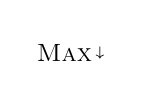
\begin{tikzpicture}[xscale=0.6,yscale=0.4]
\node (max) at (0,0) {{\small \textsc{Max}}};
\node (reg) at (0.75,0.5) {{\fns \textalpha}};
\node (arrow) at (0.75,0) {{\tiny $\downarrow$}};
\node (Rt) at (0.75,-0.5) {{\fns \textbeta}};
\end{tikzpicture}
\end{minipage}
}

\newcommand{\DepAB}{
\begin{minipage}{0.09\textwidth}
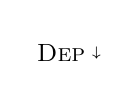
\begin{tikzpicture}[xscale=0.6,yscale=0.4]
\node (max) at (0,0) {{\small \textsc{Dep}}};
\node (reg) at (0.75,0.5) {{\fns \textalpha}};
\node (arrow) at (0.75,0) {{\tiny $\downarrow$}};
\node (Rt) at (0.75,-0.5) {{\fns \textbeta}};
\end{tikzpicture}
\end{minipage}
}

\newcommand{\DepHReg}{
\begin{minipage}{0.055\textwidth}
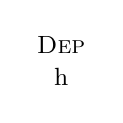
\begin{tikzpicture}[xscale=0.6,yscale=0.4]
\node (dep) at (0,0) {{\small \textsc{Dep}}};
\node (reg) at (0,-1.0) {{\small h}};
\end{tikzpicture}
\end{minipage}
}

\newcommand{\DepLReg}{
\begin{minipage}{0.055\textwidth}
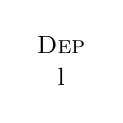
\begin{tikzpicture}[xscale=0.6,yscale=0.4]
\node (dep) at (0,0) {{\small \textsc{Dep}}};
\node (reg) at (0,-1.0) {{\small l}};
\end{tikzpicture}
\end{minipage}
}

\newcommand{\DepReg}{
\begin{minipage}{0.055\textwidth}
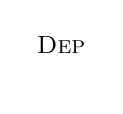
\begin{tikzpicture}[xscale=0.6,yscale=0.4]
\node (dep) at (0,0) {{\small \textsc{Dep}}};
\node (reg) at (0,-1.0) {{\small \textrho}};
\end{tikzpicture}
\end{minipage}
}

\newcommand{\DepTRt}{
\begin{minipage}{0.1\textwidth}
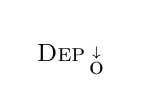
\begin{tikzpicture}[xscale=0.6,yscale=0.4]
\node (dep) at (0,0) {{\small \textsc{Dep}}};
\node (t) at (0.75,0.5) {{\fns \texttau}};
\node (arrow) at (0.75,0) {{\tiny $\downarrow$}};
\node (Rt) at (0.75,-0.5) {{\fns o}};
\end{tikzpicture}
\end{minipage}
}

\newcommand{\MaxRegRt}{
\begin{minipage}{0.1\textwidth}
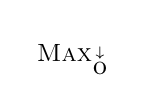
\begin{tikzpicture}[xscale=0.6,yscale=0.4]
\node (max) at (0,0) {{\small \textsc{Max}}};
\node (arrow) at (0.75,0) {{\tiny $\downarrow$}};
\node (Rt) at (0.75,-0.5) {{\fns o}};
\node (reg) at (0.75,0.5) {{\fns \textrho}};
\end{tikzpicture}
\end{minipage}
}

\newcommand{\RegToneByRt}{
\begin{minipage}{0.06\textwidth}
\begin{tikzpicture}[xscale=0.6,yscale=0.5]
\node[rotate=20] (arrow1) at (-0.15,0) {{\fns $\uparrow$}};
\node[rotate=340] (arrow2) at (0.15,0) {{\fns $\uparrow$}};
\node (Rt) at (0,-0.55) {{\small o}};
\node (reg) at (0.4,0.55) {{\small \textrho}};
\node (tone) at (-0.4,0.55) {{\small \texttau}};
\end{tikzpicture}
\end{minipage}
}

\newcommand{\RegToneBySyl}{
\begin{minipage}{0.06\textwidth}
\begin{tikzpicture}[xscale=0.6,yscale=0.5]
\node[rotate=20] (arrow1) at (-0.15,0) {{\fns $\uparrow$}};
\node[rotate=340] (arrow2) at (0.15,0) {{\fns $\uparrow$}};
\node (Rt) at (0,-0.55) {{\small \textsigma}};
\node (reg) at (0.4,0.55) {{\small \textrho}};
\node (tone) at (-0.4,0.55) {{\small \texttau}};
\end{tikzpicture}
\end{minipage}
}

\newcommand{\DepTone}{
\begin{minipage}{0.055\textwidth}
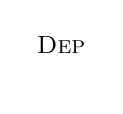
\begin{tikzpicture}[xscale=0.6,yscale=0.4]
\node (dep) at (0,0) {{\small \textsc{Dep}}};
\node (tone) at (0,-1.0) {{\small \texttau}};
\end{tikzpicture}
\end{minipage}
}

\newcommand{\DepTonalRt}{
\begin{minipage}{0.055\textwidth}
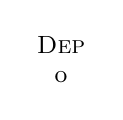
\begin{tikzpicture}[xscale=0.6,yscale=0.4]
\node (dep) at (0,0) {{\small \textsc{Dep}}};
\node (tone) at (0,-1.0) {{\small o}};
\end{tikzpicture}
\end{minipage}
}

\newcommand{\DepL}{
\begin{minipage}{0.055\textwidth}
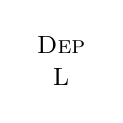
\begin{tikzpicture}[xscale=0.6,yscale=0.4]
\node (dep) at (0,0) {{\small \textsc{Dep}}};
\node (tone) at (0,-1.0) {{\small L}};
\end{tikzpicture}
\end{minipage}
}

\newcommand{\DepH}{
\begin{minipage}{0.055\textwidth}
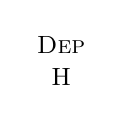
\begin{tikzpicture}[xscale=0.6,yscale=0.4]
\node (dep) at (0,0) {{\small \textsc{Dep}}};
\node (tone) at (0,-1.0) {{\small H}};
\end{tikzpicture}
\end{minipage}
}

\newcommand{\NoMultDiff}{{\small *loh}}
\newcommand{\Alt}{{\small \textsc{Alt}}}
\newcommand{\NoSkip}{{\small \scell{\textsc{No}\\\textsc{Skip}}}}


\newcommand{\RegDomRt}{
\begin{minipage}{0.030\textwidth}
\begin{tikzpicture}[xscale=0.6,yscale=0.5]
\node (arrow) at (0,0) {{\fns $\downarrow$}};
\node (Rt) at (0,-0.55) {{\small o}};
\node (reg) at (0,0.55) {{\small \textrho}};
\end{tikzpicture}
\end{minipage}
}

\newcommand{\DepRegRt}{
\begin{minipage}{0.1\textwidth}
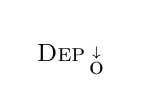
\begin{tikzpicture}[xscale=0.6,yscale=0.4]
\node (dep) at (0,0) {{\small \textsc{Dep}}};
\node (arrow) at (0.75,0) {{\tiny $\downarrow$}};
\node (Rt) at (0.75,-0.5) {{\fns o}};
\node (reg) at (0.75,0.5) {{\fns \textrho}};
\end{tikzpicture}
\end{minipage}
}

% unused

\newcommand{\ToneByRt}{
\begin{minipage}{0.05\textwidth}
\begin{tikzpicture}[xscale=0.6,yscale=0.5]
\node (arrow) at (0,0) {{\fns $\uparrow$}};
\node (Rt) at (0,-0.55) {{\small o}};
\node (tone) at (0,0.55) {{\small \texttau}};
\end{tikzpicture}
\end{minipage}
}

\newcommand{\RegByRt}{
\begin{minipage}{0.05\textwidth}
\begin{tikzpicture}[xscale=0.6,yscale=0.5]
\node (arrow) at (0,0) {{\fns $\uparrow$}};
\node (Rt) at (0,-0.55) {{\small o}};
\node (reg) at (0,0.55) {{\small \textrho}};
\end{tikzpicture}
\end{minipage}
}

\newcommand{\ToneDomRt}{
\begin{minipage}{0.05\textwidth}
\begin{tikzpicture}[xscale=0.6,yscale=0.5]
\node (arrow) at (0,0) {{\fns $\downarrow$}};
\node (Rt) at (0,-0.55) {{\small o}};
\node (tone) at (0,0.55) {{\small \texttau}};
\end{tikzpicture}
\end{minipage}
}

% --- OT tableaus --- %

% Sec. 3.2, first tabl.

\newcommand{\OTHLInput}{
\begin{minipage}{0.17\textwidth}
\begin{tikzpicture}[xscale=\myscalex,yscale=\myscaley]
\node (tone) at (2,0) {(= H)};
\node (syl) at (0,0) {\textsigma};
\node (Rt) at (0,1) {o};
\node (H) at (-0.5,2) {H};
\node (R) at (0.5,3) {h};
\node (Rt2) at (1.5,1.0) {o};
%\node (H2) at (1.0,2) {\epen{L}};
\node (R2) at (2.0,3) {\blue{l}};
\draw [thick] (syl.north) -- (Rt.south) ;
\draw [thick] (Rt.north) -- (H.south) ;
\draw [thick] (Rt.north) -- (R.south) ;
\draw [thick] (syl.north) -- (Rt2.south) ;
%\draw [dashed] (Rt2.north) -- (H2.south) ;
%\draw [dashed] (Rt2.north) -- (R2.south) ;
\end{tikzpicture}
\end{minipage}
}

\newcommand{\OTHLWinner}{
\begin{minipage}{0.17\textwidth}
\begin{tikzpicture}[xscale=\myscalex,yscale=\myscaley]
\node (tone) at (2,0) {(= HL)};
\node (syl) at (0,0) {\textsigma};
\node (Rt) at (0,1) {o};
\node (H) at (-0.5,2) {H};
\node (R) at (0.5,3) {h};
\node (Rt2) at (1.5,1.0) {o};
\node (H2) at (1.0,2) {\epen{L}};
\node (R2) at (2.0,3) {\blue{l}};
\draw [thick] (syl.north) -- (Rt.south) ;
\draw [thick] (Rt.north) -- (H.south) ;
\draw [thick] (Rt.north) -- (R.south) ;
\draw [thick] (syl.north) -- (Rt2.south) ;
\draw [dashed] (Rt2.north) -- (H2.south) ;
\draw [dashed] (Rt2.north) -- (R2.south) ;
\end{tikzpicture}
\end{minipage}
}

\newcommand{\OTHLSpreadingHOnly}{
\begin{minipage}{0.17\textwidth}
\begin{tikzpicture}[xscale=\myscalex,yscale=\myscaley]
\node (tone) at (2,0) {(= HM)};
\node (syl) at (0,0) {\textsigma};
\node (Rt) at (0,1) {o};
\node (H) at (-0.5,2) {H};
\node (R) at (0.5,3) {h};
\node (Rt2) at (1.5,1.0) {o};
%\node (H2) at (1.0,2) {\epen{L}};
\node (R2) at (2.0,3) {\blue{l}};
\draw [thick] (syl.north) -- (Rt.south) ;
\draw [thick] (Rt.north) -- (H.south) ;
\draw [thick] (Rt.north) -- (R.south) ;
\draw [thick] (syl.north) -- (Rt2.south) ;
\draw [dashed] (Rt2.north) -- (R2.south) ;
\draw [dashed] (Rt2.north) -- (H.south) ;
\end{tikzpicture}
\end{minipage}
}

\newcommand{\OTHLInsertH}{
\begin{minipage}{0.17\textwidth}
\begin{tikzpicture}[xscale=\myscalex,yscale=\myscaley]
\node (tone) at (2,0) {(= HM)};
\node (syl) at (0,0) {\textsigma};
\node (Rt) at (0,1) {o};
\node (H) at (-0.5,2) {H};
\node (R) at (0.5,3) {h};
\node (Rt2) at (1.5,1.0) {o};
\node (H2) at (1.0,2) {\epen{H}};
\node (R2) at (2.0,3) {\blue{l}};
\draw [thick] (syl.north) -- (Rt.south) ;
\draw [thick] (Rt.north) -- (H.south) ;
\draw [thick] (Rt.north) -- (R.south) ;
\draw [thick] (syl.north) -- (Rt2.south) ;
\draw [dashed] (Rt2.north) -- (H2.south) ;
\draw [dashed] (Rt2.north) -- (R2.south) ;
\end{tikzpicture}
\end{minipage}
}

\newcommand{\OTHLOverwriting}{
\begin{minipage}{0.17\textwidth}
\begin{tikzpicture}[xscale=\myscalex,yscale=\myscaley]
\node (syl) at (0,0) {\textsigma};
\node (Rt) at (0,1) {o};
\node (H) at (-0.5,2) {H};
\node (R) at (0.5,3) {h};
\node (Rt2) at (1.5,1.0) {o};
%\node (H2) at (1.0,2) {\epen{L}};
\node (R2) at (2.0,3) {\blue{l}};
\draw [thick] (syl.north) -- (Rt.south) ;
\draw [thick] (Rt.north) -- (H.south) ;
\draw [thick] (Rt.north) -- (R.south) ;
\draw [thick] (syl.north) -- (Rt2.south) ;
%\draw [dashed] (Rt2.north) -- (H2.south) ;
\draw [dashed] (Rt.north) -- (R2.south) ;
\node (del) at (0.3,1.9) {\textbf{=}};
\end{tikzpicture}
\end{minipage}
}

\newcommand{\OTHLSpreading}{
\begin{minipage}{0.17\textwidth}
\begin{tikzpicture}[xscale=\myscalex,yscale=\myscaley]
\node (syl) at (0,0) {\textsigma};
\node (Rt) at (0,1) {o};
\node (H) at (-0.5,2) {H};
\node (R) at (0.5,3) {h};
\node (Rt2) at (1.5,1.0) {o};
%\node (H2) at (1.0,2) {\epen{L}};
\node (R2) at (2.0,3) {\blue{l}};
\draw [thick] (syl.north) -- (Rt.south) ;
\draw [thick] (Rt.north) -- (H.south) ;
\draw [thick] (Rt.north) -- (R.south) ;
\draw [thick] (syl.north) -- (Rt2.south) ;
%\draw [dashed] (Rt2.north) -- (H2.south) ;
\draw [dashed] (Rt2.north) -- (H.south) ;
\draw [dashed] (Rt2.north) -- (R.south) ;
\end{tikzpicture}
\end{minipage}
}

% Sec. 4.2, second tabl.: phrase-medial position

\newcommand{\OTHnoLInput}{
\begin{minipage}{0.17\textwidth}
\begin{tikzpicture}[xscale=\myscalex,yscale=\myscaley]
\node (tone) at (2,0) {(= H)};
\node (syl) at (0,0) {\textsigma};
\node (Rt) at (0,1) {o};
\node (H) at (-0.5,2) {H};
\node (R) at (0.5,3) {h};
\node (Rt2) at (1.5,1.0) {o};
%\node (H2) at (1.0,2) {\epen{L}};
%\node (R2) at (2.0,3) {\blue{l}};
\draw [thick] (syl.north) -- (Rt.south) ;
\draw [thick] (Rt.north) -- (H.south) ;
\draw [thick] (Rt.north) -- (R.south) ;
\draw [thick] (syl.north) -- (Rt2.south) ;
\end{tikzpicture}
\end{minipage}
}

\newcommand{\OTHnoLEpenth}{
\begin{minipage}{0.17\textwidth}
\begin{tikzpicture}[xscale=\myscalex,yscale=\myscaley]
\node (tone) at (2,0) {(= HM)};
\node (syl) at (0,0) {\textsigma};
\node (Rt) at (0,1) {o};
\node (H) at (-0.5,2) {H};
\node (R) at (0.5,3) {h};
\node (Rt2) at (1.5,1.0) {o};
\node (H2) at (1.0,2) {\epen{L}};
\node (R2) at (2.0,3) {\epen{h}};
\draw [thick] (syl.north) -- (Rt.south) ;
\draw [thick] (Rt.north) -- (H.south) ;
\draw [thick] (Rt.north) -- (R.south) ;
\draw [thick] (syl.north) -- (Rt2.south) ;
\draw [dashed] (Rt2.north) -- (H2.south) ;
\draw [dashed] (Rt2.north) -- (R2.south) ;
\end{tikzpicture}
\end{minipage}
}

\newcommand{\OTHnoLSpreading}{
\begin{minipage}{0.17\textwidth}
\begin{tikzpicture}[xscale=\myscalex,yscale=\myscaley]
\node (tone) at (2,0) {(= HH)};
\node (syl) at (0,0) {\textsigma};
\node (Rt) at (0,1) {o};
\node (H) at (-0.5,2) {H};
\node (R) at (0.5,3) {h};
\node (Rt2) at (1.5,1.0) {o};
%\node (H2) at (1.0,2) {\epen{L}};
%\node (R2) at (2.0,3) {\blue{l}};
\draw [thick] (syl.north) -- (Rt.south) ;
\draw [thick] (Rt.north) -- (H.south) ;
\draw [thick] (Rt.north) -- (R.south) ;
\draw [thick] (syl.north) -- (Rt2.south) ;
\draw [dashed] (Rt2.north) -- (H.south) ;
\draw [dashed] (Rt2.north) -- (R.south) ;
\end{tikzpicture}
\end{minipage}
}

% Sec. 4.2, third tabl., LM is unaffected by L\%

\newcommand{\OTLMInput}{
\begin{minipage}{0.2\textwidth}
\begin{tikzpicture}[xscale=\myscalex,yscale=\myscaley]
\node (tone) at (2,0) {(= LM)};
\node (syl) at (0,0) {\textsigma};
\node (Rt) at (0,1) {o};
\node (H) at (-0.5,2) {L};
\node (R) at (0.5,3) {l};
\node (Rt2) at (1.5,1.0) {o};
\node (H2) at (1.0,2) {L};
\node (R2) at (2.0,3) {h};
\node (R3) at (3.0,3) {\blue{l}};
\draw [thick] (syl.north) -- (Rt.south) ;
\draw [thick] (Rt.north) -- (H.south) ;
\draw [thick] (Rt.north) -- (R.south) ;
\draw [thick] (syl.north) -- (Rt2.south) ;
\draw [thick] (Rt2.north) -- (H2.south) ;
\draw [thick] (Rt2.north) -- (R2.south) ;
\end{tikzpicture}
\end{minipage}
}

\newcommand{\OTLMReplace}{
\begin{minipage}{0.2\textwidth}
\begin{tikzpicture}[xscale=\myscalex,yscale=\myscaley]
\node (tone) at (2,0) {(= LL)};
\node (syl) at (0,0) {\textsigma};
\node (Rt) at (0,1) {o};
\node (H) at (-0.5,2) {L};
\node (R) at (0.5,3) {l};
\node (Rt2) at (1.5,1.0) {o};
\node (H2) at (1.0,2) {L};
\node (R2) at (2.0,3) {h};
\node (R3) at (3.0,3) {\blue{l}};
\draw [thick] (syl.north) -- (Rt.south) ;
\draw [thick] (Rt.north) -- (H.south) ;
\draw [thick] (Rt.north) -- (R.south) ;
\draw [thick] (syl.north) -- (Rt2.south) ;
\draw [thick] (Rt2.north) -- (H2.south) ;
\draw [thick] (Rt2.north) -- (R2.south) ;
\draw [dashed] (Rt2.north) -- (R3.south) ;
\node (del) at (1.8,2.1) {\textbf{=}};
\end{tikzpicture}
\end{minipage}
}

\newcommand{\OTLMTwoReg}{
\begin{minipage}{0.2\textwidth}
\begin{tikzpicture}[xscale=\myscalex,yscale=\myscaley]
\node (tone) at (2,0) {(= LML)};
\node (syl) at (0,0) {\textsigma};
\node (Rt) at (0,1) {o};
\node (H) at (-0.5,2) {L};
\node (R) at (0.5,3) {l};
\node (Rt2) at (1.5,1.0) {o};
\node (H2) at (1.0,2) {L};
\node (R2) at (2.0,3) {h};
\node (R3) at (3.0,3) {\blue{l}};
\draw [thick] (syl.north) -- (Rt.south) ;
\draw [thick] (Rt.north) -- (H.south) ;
\draw [thick] (Rt.north) -- (R.south) ;
\draw [thick] (syl.north) -- (Rt2.south) ;
\draw [thick] (Rt2.north) -- (H2.south) ;
\draw [thick] (Rt2.north) -- (R2.south) ;
\draw [dashed] (Rt2.north) -- (R3.south) ;
\end{tikzpicture}
\end{minipage}
}

% Sec. 4.2, fourth tabl., L is affected by L\% but M is not

\newcommand{\OTLInput}{
\begin{minipage}{0.17\textwidth}
\begin{tikzpicture}[xscale=\myscalex,yscale=\myscaley]
\node (tone) at (2,0) {(= L)};
\node (syl) at (0,0) {\textsigma};
\node (Rt) at (0,1) {o};
\node (H) at (-0.5,2) {L};
\node (R) at (0.5,3) {l};
\node (R2) at (2,3) {\blue{l}};
\draw [thick] (syl.north) -- (Rt.south) ;
\draw [thick] (Rt.north) -- (H.south) ;
\draw [thick] (Rt.north) -- (R.south) ;
\end{tikzpicture}
\end{minipage}
}

\newcommand{\OTLLowered}{
\begin{minipage}{0.17\textwidth}
\begin{tikzpicture}[xscale=\myscalex,yscale=\myscaley]
\node (tone) at (2,0) {(= LL)};
\node (syl) at (0,0) {\textsigma};
\node (Rt) at (0,1) {o};
\node (H) at (-0.5,2) {L};
\node (R) at (0.5,3) {l};
\node (R2) at (2,3) {\blue{l}};
\draw [thick] (syl.north) -- (Rt.south) ;
\draw [thick] (Rt.north) -- (H.south) ;
\draw [thick] (Rt.north) -- (R.south) ;
\draw [dashed] (Rt.north) -- (R2.south) ;
\end{tikzpicture}
\end{minipage}
}

\newcommand{\OTMInput}{
\begin{minipage}{0.17\textwidth}
\begin{tikzpicture}[xscale=\myscalex,yscale=\myscaley]
\node (tone) at (2,0) {(= M)};
\node (syl) at (0,0) {\textsigma};
\node (Rt) at (0,1) {o};
\node (H) at (-0.5,2) {L};
\node (R) at (0.5,3) {h};
\node (R2) at (2,3) {\blue{l}};
\draw [thick] (syl.north) -- (Rt.south) ;
\draw [thick] (Rt.north) -- (H.south) ;
\draw [thick] (Rt.north) -- (R.south) ;
\end{tikzpicture}
\end{minipage}
}

\newcommand{\OTMLowered}{
\begin{minipage}{0.17\textwidth}
\begin{tikzpicture}[xscale=\myscalex,yscale=\myscaley]
\node (tone) at (2,0) {(= ML)};
\node (syl) at (0,0) {\textsigma};
\node (Rt) at (0,1) {o};
\node (H) at (-0.5,2) {L};
\node (R) at (0.5,3) {h};
\node (R2) at (2,3) {\blue{l}};
\draw [thick] (syl.north) -- (Rt.south) ;
\draw [thick] (Rt.north) -- (H.south) ;
\draw [thick] (Rt.north) -- (R.south) ;
\draw [dashed] (Rt.north) -- (R2.south) ;
\end{tikzpicture}
\end{minipage}
}

% Sec. 4.2, fifth tableau, polar questions with level tones

\newcommand{\OTLPolIn}{
\begin{minipage}{0.20\textwidth}
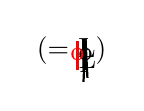
\begin{tikzpicture}[xscale=\myscalex-0.05,yscale=\myscaley-0.05]
\node (tone) at (3.5,0) {(= L)};
\node (syl) at (0,0) {\textsigma};
\node (syl2) at (2,0) {\red{\textsigma}};
\node (Rt) at (0,1) {o};
\node (H) at (-0.5,2) {L};
\node (R) at (0.5,3) {l};
\node (Rt2) at (2,1) {\red{o}};
\draw [thick] (syl.north) -- (Rt.south) ;
\draw [thick,red] (syl2.north) -- (Rt2.south) ;
\draw [thick] (Rt.north) -- (H.south) ;
\draw [thick] (Rt.north) -- (R.south) ;
\end{tikzpicture}
\end{minipage}
}

\newcommand{\OTLPolDef}{
\begin{minipage}{0.20\textwidth}
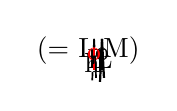
\begin{tikzpicture}[xscale=\myscalex-0.05,yscale=\myscaley-0.05]
\node (tone) at (3.5,0) {(= L.M)};
\node (syl) at (0,0) {\textsigma};
\node (syl2) at (2,0) {\red{\textsigma}};
\node (Rt) at (0,1) {o};
\node (H) at (-0.5,2) {L};
\node (R) at (0.5,3) {l};
\node (H2) at (1.5,2) {\epen{L}};
\node (R2) at (2.5,3) {\epen{h}};
\node (Rt2) at (2,1) {\red{o}};
\draw [thick] (syl.north) -- (Rt.south) ;
\draw [thick,red] (syl2.north) -- (Rt2.south) ;
\draw [thick] (Rt.north) -- (H.south) ;
\draw [thick] (Rt.north) -- (R.south) ;
\draw [semithick,dashed] (Rt2.north) -- (H2.south) ;
\draw [semithick,dashed] (Rt2.north) -- (R2.south) ;
\end{tikzpicture}
\end{minipage}
}

\newcommand{\OTLPolAlt}{
\begin{minipage}{0.20\textwidth}
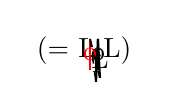
\begin{tikzpicture}[xscale=\myscalex-0.05,yscale=\myscaley-0.05]
\node (tone) at (3.5,0) {(= L.L)};
\node (syl) at (0,0) {\textsigma};
\node (syl2) at (2,0) {\red{\textsigma}};
\node (Rt) at (0,1) {o};
\node (H) at (-0.5,2) {L};
\node (R) at (0.5,3) {l};
\node (Rt2) at (2,1) {\red{o}};
\draw [thick] (syl.north) -- (Rt.south) ;
\draw [thick,red] (syl2.north) -- (Rt2.south) ;
\draw [thick] (Rt.north) -- (H.south) ;
\draw [thick] (Rt.north) -- (R.south) ;
\draw [semithick,dashed] (Rt2.north) -- (H.south) ;
\draw [semithick,dashed] (Rt2.north) -- (R.south) ;
\end{tikzpicture}
\end{minipage}
}

% Sec. 4.2, sixth tableau, polar questions with contour tones

\newcommand{\OTLLPolIn}{
\begin{minipage}{0.23\textwidth}
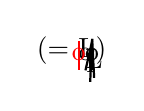
\begin{tikzpicture}[xscale=\myscalex-0.05,yscale=\myscaley-0.05]
\node (tone) at (5.2,0) {(= L)};
\node (syl) at (0,0) {\textsigma};
\node (syl3) at (3.4,0) {\red{\textsigma}};
\node (Rt) at (0,1) {o};
\node (Rt2) at (1.7,1) {o};
\node (Rt3) at (3.4,1) {\red{o}};
\node (H) at (-0.5,2) {L};
\node (R) at (0.5,3) {l};
\draw [thick] (syl.north) -- (Rt.south) ;
\draw [thick] (syl.north) -- (Rt2.south) ;
\draw [thick,red] (syl3.north) -- (Rt3.south) ;
\draw [thick] (Rt.north) -- (H.south) ;
\draw [thick] (Rt.north) -- (R.south) ;
\end{tikzpicture}
\end{minipage}
}

\newcommand{\OTLLPolDef}{
\begin{minipage}{0.23\textwidth}
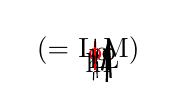
\begin{tikzpicture}[xscale=\myscalex-0.05,yscale=\myscaley-0.05]
\node (tone) at (5.2,0) {(= L.M)};
\node (syl) at (0,0) {\textsigma};
\node (syl3) at (3.4,0) {\red{\textsigma}};
\node (Rt) at (0,1) {o};
\node (Rt2) at (1.7,1) {o};
\node (Rt3) at (3.4,1) {\red{o}};
\node (H) at (-0.5,2) {L};
\node (R) at (0.5,3) {l};
\node (H3) at (2.9,2) {\epen{L}};
\node (R3) at (3.9,3) {\epen{h}};
\draw [thick] (syl.north) -- (Rt.south) ;
\draw [thick] (syl.north) -- (Rt2.south) ;
\draw [thick,red] (syl3.north) -- (Rt3.south) ;
\draw [thick] (Rt.north) -- (H.south) ;
\draw [thick] (Rt.north) -- (R.south) ;
\draw [dashed] (Rt3.north) -- (H3.south) ;
\draw [dashed] (Rt3.north) -- (R3.south) ;
\end{tikzpicture}
\end{minipage}
}

\newcommand{\OTLLPolSkip}{
\begin{minipage}{0.23\textwidth}
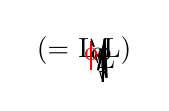
\begin{tikzpicture}[xscale=\myscalex-0.05,yscale=\myscaley-0.05]
\node (tone) at (5.2,0) {(= L.L)};
\node (syl) at (0,0) {\textsigma};
\node (syl3) at (3.4,0) {\red{\textsigma}};
\node (Rt) at (0,1) {o};
\node (Rt2) at (1.7,1) {o};
\node (Rt3) at (3.4,1) {\red{o}};
\node (H) at (-0.5,2) {L};
\node (R) at (0.5,3) {l};
\draw [thick] (syl.north) -- (Rt.south) ;
\draw [thick] (syl.north) -- (Rt2.south) ;
\draw [thick,red] (syl3.north) -- (Rt3.south) ;
\draw [thick] (Rt.north) -- (H.south) ;
\draw [thick] (Rt.north) -- (R.south) ;
\draw [dashed] (Rt3.north) -- (H.south) ;
\draw [dashed] (Rt3.north) -- (R.south) ;
\end{tikzpicture}
\end{minipage}
}  
  
\newcommand{\ilit}[1]{#1\il{#1}}    
\newcommand{\isit}[1]{#1\is{#1}}  

\makeatletter
\let\thetitle\@title
\let\theauthor\@author 
\makeatother

\newcommand{\togglepaper}[1][0]{ 
  \bibliography{../localbibliography}
  %% hyphenation points for line breaks
%% Normally, automatic hyphenation in LaTeX is very good
%% If a word is mis-hyphenated, add it to this file
%%
%% add information to TeX file before \begin{document} with:
%% %% hyphenation points for line breaks
%% Normally, automatic hyphenation in LaTeX is very good
%% If a word is mis-hyphenated, add it to this file
%%
%% add information to TeX file before \begin{document} with:
%% \include{localhyphenation}
\hyphenation{
affri-ca-te
affri-ca-tes
com-ple-ments
par-a-digm
Sha-ron
Kings-ton
phe-nom-e-non
Daul-ton
Abu-ba-ka-ri
Ngo-nya-ni
Clem-ents 
King-ston
Tru-cken-brodt
Tab-leau
cophono-logies
mark-edness
Ti-gri-nya
a-mong
Car-stens
Lu-bu-ku-su
}
\hyphenation{
affri-ca-te
affri-ca-tes
com-ple-ments
par-a-digm
Sha-ron
Kings-ton
phe-nom-e-non
Daul-ton
Abu-ba-ka-ri
Ngo-nya-ni
Clem-ents 
King-ston
Tru-cken-brodt
Tab-leau
cophono-logies
mark-edness
Ti-gri-nya
a-mong
Car-stens
Lu-bu-ku-su
}
  \papernote{\scriptsize\normalfont
    \theauthor.
    \thetitle. 
    To appear in: 
    Emily Clem,   Peter Jenks \& Hannah Sande.
    Theory and description in African Linguistics: Selected papers from the 47th Annual Conference on African Linguistics.
    Berlin: Language Science Press. [preliminary page numbering]
  }
  \pagenumbering{roman}
  \setcounter{chapter}{#1}
  \addtocounter{chapter}{-1}
}

\newcommand{\upstep}{\textupstep}


% \newcounter{tableauxcounter}

\renewcommand{\textltailn}{ɲ}
\renewcommand{\textbardotlessj}{ɟ}

\newcommand{\emphkh}[1]{\textit{#1}} %originally \textbf, banned by the guidelines



\definecolor{lsDOIGray}{cmyk}{0,0,0,0.45}


\newcommand{\xuparrow}[1]{%
  {\left\uparrow\vbox to #1{}\right.\kern-\nulldelimiterspace}
}
\renewcommand \textupstep[1]{\char"A71B#1}
\renewcommand \textdownstep[1]{\char"A71C#1}
 
 \newcommand{\ꜛ}{\textsf{ꜛ}}
 
\def\biberror{\undefined}


\newcommand{\OTbox}[1]{\resizebox{.88\textwidth}{!}{#1}}
 

\author{Pius W. Akumbu\affiliation{University of Buea, Cameroon}}
\title{A featural analysis of mid and downstepped high tone in Babanki} 


\abstract{In this study, I examine the occurrence of the surface Mid (M) and downstepped High (↓H) tone in Babanki, a Central Ring Grassfields Bantu language of Cameroon. \citet{Hyman1979babanki} has demonstrated that Babanki has two underlying tones, namely, High (H) and Low (L), and that on the surface, it contrasts three level tones, H, M, L, plus a downstepped High (↓H). There is also contrast between a falling (L) and a level low (Lo) tone before pause in the language. I demonstrate in this paper that the M tone is from two different phonological sources and derived by the regressive spread of the high register feature of a following H tone while ↓H is caused by the progressive spread of the low register feature of a preceding floating L tone. The M and ↓H tone are phonetically identical in the language but differ in that ↓H establishes a ceiling for following H tones within the same tonal phrase.
}
\newtier{top,bot,reg}
\psset{everyasr=\tiershortcuts,
 ph=0,ts=0,top=(ph) 4 1.5em 0.5em,bot=(ph) -3 1em 1em,reg=(ph) -6 1em 1em,botB=-1.5,topB=4.5,regB=-3.5,phht=2.5ex}
\begin{document}

\maketitle

\section{Introduction}

Part of the complexity of \isi{tone} in \ili{Grassfields} \ili{Bantu} (GB) languages of Northwest Cameroon such as \ili{Babanki} (a Central \ili{Ring} GB language) is the lack of correspondence between underlying and surface tones as well as the presence of many floating tones. There is no underlying M \isi{tone} in \ili{Babanki}, yet it occurs on the surface with the constraint that it must be followed by a H \isi{tone}. \citet[][]{Hyman1979babanki} has given a historical account of this M \isi{tone} which is unnecessarily abstract as a synchronic analysis. I demonstrate in this paper that M \isi{tone} results from the regressive spread of the [+R] feature of high tones which is blocked only by a nasal in NC initial roots. Downstep on its part results from the progressive spread of the [\textminus R] feature of a floating L \isi{tone}. The synchronic reanalysis of \ili{Babanki} surface tones in this paper addresses the following issues: 1) What are the underlying sources of the M \isi{tone}? 2) How should the M \isi{tone} be represented, as opposed to the downstepped H? I begin by illustrating in §2 that the lexical tones of \ili{Babanki} are H and L even though a number of other tonal distinctions are found on the surface. I then proceed to examine the sources of M \isi{tone} in the language in §3 before turning to discuss how the M \isi{tone} is derived in §4. In §5, I provide evidence that both M and ↓H are phonetically identical and differ only in that the \isi{register} is reset to high after M \isi{tone} but not after ↓H which establishes a ceiling for future H tones within the same tonal phrase.

\section{Babanki lexical tone}
\ili{Babanki} has two underlying tones, namely H and L, illustrated in (1). As a native speaker, I have provided most of the data but have also taken some from prior literature, particularly \citet{Hyman1979babanki} and a lexical database of 2,005 \ili{Babanki} entries in Filemaker Pro™.\footnote{The IPA symbols for the following orthographic symbols used in this paper are given in square brackets: ny [ɲ], sh [ʃ], zh [ʒ], gh [gh], ch [tʃ], j [dʒ], y [j].}

\ea\label{ex:akumba:1}
\downingquad{{ndɔ̀ŋ}}{‘potato’}{{ndɔ́ŋ}}{‘cup’}
\downingquad{{kə̀-bwìn}}{‘witchcraft’}{kə̀-bwín}{‘ridge’}
\downingquad{{ə̀-sè}}{‘grave’}{{ə̀-sé}}{‘profit(n)’}
\downingquad{{kə̀-mbò}}{‘bag’}{{kə̀-mbó}}{‘madness’}
\z

On the surface, however, several tonal realizations are possible. As noted by \citet[160-161]{Hyman1979babanki}, there is a distinction between falling low (L) and level low (Lo) tones before pause as in (2):
%TODO Ask what to do about this positioning
\ea\label{ex:akumba:2}
\downingquint{L}{\-}{L$\textsuperscript{o}$}{}{}
\downingquint{{kə̀-ntò}}{‘cross (n)’}{{kə̀-mbò}$\textsuperscript{o}$}{‘bag’}{/kə̀-mbòˊ/}
\downingquint{\textit{nyàm}}{‘animal’	}{\textit{dzə̀m}$\textsuperscript{o}$}{‘back’}{/dzə̀mˊ/}
\downingquint{{tàn}}{‘five’}{{wàn}$\textsuperscript{o}$}{‘child’}{/wànˊ/}
\downingquint{{ə̀-sè}}{‘grave’}{{dzè}$\textsuperscript{o}$}{‘kind of fruit’}{/dzèˊ/}
\z

The level low \isi{tone} is considered an effect of a floating high \isi{tone} that follows the low \isi{tone} and prevents it from falling.  A mid (M) \isi{tone} also occurs even though with an unusual constraint that it must be followed by a H \isi{tone}: 

\ea\label{ex:akumba:3}
\ea\label{ex:akumba:3a}
			{káŋ fə̄sɛ́s}\footnote{There is a change in the root vowel because in \ili{Babanki}, /e/ and /o/ are realized as [ɛ] and [ɔ] respectively in closed syllables \citep[75]{Mutaka2006}.}\\		
\gll		{káŋ} 	ˊ	{fə̀-sés}\\
			fry	IMP 	c19-pepper\\
\glt		‘fry pepper’ 

\ex\label{ex:akumba:3b}
			{kùmə́ kə̄kɨ́}		\\
\gll		{kùm}	ˊ	{kə̀-kɨ́}\\
			touch	IMP	c7-chair\\
\glt		‘touch a chair’

\ex\label{ex:akumba:3c}
			{gháʔ kə̄vú}	\\	
\gll		{gháʔ} 	ˊ	{kə̀-vu}́\\
			hold	IMP	c7-hand\\
\glt		‘hold a hand’
\z
\z

The data show that the M \isi{tone} is derived from a L \isi{tone} found between two H tones as illustrated in §3.1 and discussed elaborately in §4.  Finally, there is a downstepped H \isi{tone} as in (4):

\ea\label{ex:akumba:4}
\ea\label{ex:akumba:4a}
		{kə̀-fóˋ ↓kə́ nyàm }	\\
\gll		{kə̀-fóˋ}		{kə}́ 	{nyàm}\\
		c7-thing	AM	c9-animal\\
\glt		‘thing of animal’

\ex\label{ex:akumba:4b}
		{kə̀mbó ↓kə́ wìʔ}	\\
\gll		{kə̀-mbóˋ} 	{kə́ }	{wìʔ}\\
		c7-madness	AM	c1.person\\
\glt		‘madness of person’

\ex\label{ex:akumba:4c}
		{kə̀káŋ ↓kə́ byí shɔ́m}	\\
\gll		{kə̀-káŋˋ} 	{kə́} 	{byí} 		{shɔ́m}	\\
		c7-dish	AM	goat.c10	mine.c10	\\
\glt		‘dish of my goats’ 
\z
\z

The data in (4) illustrate that the H \isi{tone} of the associative marrker (\textsc{am}) is produced at a lower level than that of the preceding noun root because of the intervening floating L \isi{tone}. This is discussed further and formalized in §5. 
The presence of both M and ↓H in the same language is of interest for two reasons. First, \ili{Babanki} is unique in that \ili{Grassfields} \ili{Bantu} \ili{Ring} languages are typically said to have either M or ↓H. As Hyman puts it: 
\begin{quote}
	For example, it is known that the western \ili{Ring} languages and \ili{Babanki} (of the central \ili{Ring} group) have similar downstep systems. The remaining languages of the central group (\ili{Kom}, Bum, Bafmeng, Oku, Mbizinaku) all have systems with M \isi{tone} instead of ↓H, a system which \citet{Grebe1975} have also documented for \ili{Lamnsoq} of the eastern group \citep[176-177]{Hyman1979babanki}.
\end{quote}

Second, although phonologically distinct, the M and ↓H tones are phonetically identical, as I shall show below, which is of particular interest to the study of \isi{tone} in general. It is therefore necessary to examine how the M \isi{tone} is derived and how it should be formally represented. 

It is important to note that contour tones are rare in the language, allowed mainly in a few borrowed words. In the lexical database of 2,005 \ili{Babanki} entries in Filemaker Pro™, only eight monosyllabic nouns with low-Rising (LH) and four with high-falling (HL) tones were found.\footnote{LH: \textit{àŋkʉ̌ɲàm} ‘pig’, \textit{bə̌lə̀ŋ} ‘groundnut’, \textit{fə̀ndzǒndzò} ‘type of bird’, \textit{kə̀ŋgǔ} ‘fool (n)’, \textit{mbwǐ} ‘nail’, \textit{ŋgǔ} ‘rake (n)’, \textit{sǒ} ‘saw (n)’, \textit{tǒlʉ̀m} ‘cobra’.\\
HL: \textit{bɨ̂bɨ̀} ‘deaf’, \textit{bôbó} ‘Lord’, \textit{byə̂} ‘pear’, \textit{lâm} ‘lamp’, \textit{kî} ‘key’, \textit{chôs} ‘church’, \textit{wâs} ‘watch’. \\
The presence of words like \textit{sǒ} ‘saw (n)’, \textit{lâm} ‘lamp’, etc. 
suggests that many of the \ili{Babanki} words with contour tones are borrowings.}

\section{Sources of Babanki M tone}

The M \isi{tone} is derived in \ili{Babanki} from L via two separate processes which I will refer to as prefix L-Raising and stem L-Raising.

\subsection{Prefix L-Raising: H \# L-H $→$ H \# M-H}

The L \isi{tone} of a prefix is raised to M if it appears between two H tones as in the following examples. 

%TODO Ask if I should keep the a1 a2 b1 b2 enumeration or keep as is

\ea\label{ex:akumbu:5}
\ea\label{ex:akumbu:5a}
		{tə̀tɔ́ʔ tə̄táʔ	}\\
\gll		{tə̀-tóʔ} 	{tə̀-táʔ}\\
			c13-bush	c13-three\\
\glt		‘three bushes’
		
\ex\label{ex:akumbu:5b}
		{kə̀kɨ́m kə́ və̄tsɔ́ŋ}	\\
\gll		{kə̀-kɨ́m} 	{kə́} 	{və̀-tsóŋ}\\
			c7-crab	AM	c2-thief\\
\glt		‘crab of thieves’

\ex\label{ex:akumbu:5c}
		{tə̀tɔ́ʔ tə̀bò}	\\
\gll		{tə̀-tóʔ} 	{tə̀-bò}\\
			c13-bush	c13-two\\
\glt		‘two bushes’

\ex\label{ex:akumbu:5d}
		{kə̀kɨ́m kə́ və̀lə̀mə̀}	\\
\gll		{kə̀-kɨ́m }	{kə́ }	{və̀-lə̀mə̀}		\\
			c7-crab	AM	c2-sibling\\
\glt		‘crab of siblings’
\z
\z

Raising applies in (5a) where the L is flanked by Hs but not in (5b) where it is followed by a L \isi{tone}. I return to the issue in §4 to provide a featural analysis of the raising.

\subsection{Stem L-Raising: L-L \# H → L-M \# H }

In \ili{Babanki}, the L \isi{tone} of certain noun roots that also have a L prefix is realized as M if it is followed by a H \isi{tone}. The following sets of data show stem L-Raising when the noun is in N1 position in an associative N1 of N2 construction (6a), when the noun is followed by a modifier (6b), and in verb phrases (6c). Forms without raising (i.e. with surface L \isi{tone}) are given in (6d):

\ea\label{ex:akumbu:6}
\ea\label{ex:akumbu:6a}
			{kə̀kɔ̄s kə́ wìʔ}	 \\
\gll		{kə̀-kòs} 	{kə́ }	{wìʔ}	\\ 
			c7-slave	AM	c1.person \\
\glt		‘slave of person’

\ex\label{ex:akumbu:6b}
			{fə̀kɔ̄ʔ fə́ nyàm}		 \\
\gll		{fə̀-kòʔ }		{fə́ }	{nyàm}\\
			c19-wood	AM	c9.animal	\\
\glt		‘wood of person’

\ex\label{ex:akumbu:6c}
			{fə̀sō fə́↓wɛ́n}		\\
\gll   		{fə̀-sò}		{fə́}	{wén}\\
			c19-abscess	AM	him\\
\glt		‘his abscess’

\ex\label{ex:akumbu:6d}
			{kə̀kyē lá kə̀mùʔ}	 \\
\gll		{kə̀-kyè} 	{lá} 	{kə̀-mùʔ}\\
			c7-basket	just	c7-one\\
\glt		‘just one basket’

\ex\label{ex:akumbu:6e}
			{wyé kə̀zhwī tsú}		\\
\gll		{wyé} 	{kə̀-zhwì}	{tsú}\\
			put	c7-air		there\\
\glt		‘inflate it’

\ex\label{ex:akumbu:6f}
			{kú kə̀lāŋ lúwɛ̀n}	\\
\gll		{kú} 	{kə̀-làŋ} 	{lúwèn}\\
			give	c7-cocoyam	now\\
\glt		‘give cocoyam now’

\ex\label{ex:akumbu:6g}
			{nyàm ə̀ wìʔ}	 \\
\gll		{nyàm}		{ə̀} 	{wìʔ}	 \\
			c9.animal	AM	c1.person\\ 
\glt		‘animal of person’

\ex\label{ex:akumbu:6h}
			{kə̀kɔ̀s kə̀ mùʔ}	 \\
\gll		{kə̀-kòs} 	{kə̀-mùʔ}	 \\
			c7-slave	c7-one \\
\glt		‘one slave’

\ex\label{ex:akumbu:6i}
			{ə́shù kə̀làŋ nə̀ mú↓ú	}	\\
\gll    		{ə́-shù }		{kə̀-làŋ} 	{nə̀} 	{múú}\\
			INF-wash	c7-cocoyam	PREP	c6a.water\\
\glt		‘to wash cocoyam with water’
\z
\z

To account for the raising in (6a-c), \citet[168]{Hyman1979babanki} offers a synchronic analysis which mirrors the historical developments, as in (7): 

\ea\label{ex:akumbu:7}
kə́kɔ̀s kə́ →	kə́kɔ̂s kə́ →	kə̀kɔ̂s kə́ →	kə̀kɔ̄s kə́ …
\z

As seen, the prefix originally had a H \isi{tone} which spreads onto the L \isi{tone} stem.\footnote{ Hyman’s pre-autosegmental analysis also posits a floating L after the L stem, i.e., /-kòs`/ ‘slave’. This is ignored here because it is unnecessary and also an OCP violation.} After spreading, the prefix H changes to L and then the resulting L-HL \# H sequence becomes L-M \# H by contour simplification. While this historical account derives the correct output, it appears to be unnecessarily abstract as a synchronic analysis. Instead, the H \isi{tone} on the prefix can rather be analyzed as L \citep{Akumbu2011} and the change from L to M can be accounted for as a raising rule (see §4). There is, however, a complication that either analysis must deal with: L-L nouns that have a nasal as part of the root initial NC do not become L-M before H as illustrated in (8): 

\ea\label{ex:akumbu:8}
\ea\label{ex:akumbu:8a}
			{kə̀ndɔ̀ŋ kə́ nyàm}	\\
\gll		{kə̀-ndòŋ}	{kə́}	{nyàm}\\
			c7-neck	AM	c9.animal\\
\glt		‘neck of animal’	

\ex\label{ex:akumbu:8b}
			{tə̀ŋkə̀ŋ tə́ ŋkə̀ʔ} 	\\
\gll		{tə̀-ŋkə̀ŋ} 	{tə́} 	{ŋkə̀ʔ}\\
			c13-comb	AM	c1.rooster\\
\glt		‘combs of rooster’

\ex\label{ex:akumbu:8c}
			{fə̀ŋgə̀m} {fə́} {wìʔ} 	\\
\gll		fə̀-ŋgə̀m 	fə́ 	wìʔ \\
			c19-gong	AM	c1.person   \\
\glt		‘gong of person’
\z
\z

To account for this, \citet[167]{Hyman1979babanki} distinguished two classes of nouns based on whether the stem syllable has an oral (O) or nasal (N) onset and observed that “a noun in the O class changes from L-L to L-M when in the N1 position before a H \isi{tone} associative marker. A noun in the N class \ldots remains L-L.” He illustrates that L-Raising is blocked when the N1 is from a nasal class and posits that “in N1 position, N L-L nouns and L-Lo nouns have an underlying L prefix, rather than the underlying H proposed for other noun prefixes” (Hyman 1979: 169).  Since HTS does not occur, there is no L-HL \# H sequence to become L-M \# H. While that analysis is historically plausible, we can again propose a more concrete analysis by which L-Raising is simply blocked when a L \isi{tone} root has an NC onset. As argued in \citet[9]{Akumbu2011}, there is a L \isi{tone} linked to the N in NC sequences that blocks the raising. This is because in these cases, the nasal forms part of the root and bears the same L like the root vowel because of the OCP \citep{Snider1999} that is enforced morpheme-internally in \ili{Babanki}. The multiple linking of the L (to the nasal and root vowel) violates the condition for raising, namely, that the \isi{tone} that precedes the target L must be singly-linked \citep[6]{Akumbu2011}. L-Raising will automatically not apply to L-L˚ nouns since they have a floating H after them that prevents raising from occurring.
	The fact that the roots in (8) all end with a nasal could be relevant in providing a possibility of tying the failure of L-Raising to apply to some phonetic motivation. A possibility might be that the extra nasal, an extra mora, gives the L \isi{tone} more of a chance to manifest itself. If so, then we might expect the same if the stem has a long vowel (another manifestation of an extra mora). Unfortunately, \ili{Babanki} does not have long vowels and two other problems exist: there are stems, e.g. \textit{fə̀ŋgùʔ fə́ wìʔ} ‘small stone of person’, without final nasal that do not also become M, as well as stems with final nasal, e.g. \textit{kə̀būm kə́ wìʔ} ‘mucus of person’, that do in fact become M. 
	So far, the two sources of M \isi{tone} have been presented: prefix L becomes M between Hs and stem L becomes M when preceded by a L prefix and followed by a H. It should be noted that this occurs over a word boundary although it is still unclear what the influence of the boundary is. In addition, there is another context in which a stem L becomes M. This arises when a coda consonant is deleted intervocalically (see \citealt{akumbu2016} and references cited therein for more information on coda deletion in \ili{Babanki}). As seen in (9), when the CVC stem is H and the following prefix vowel is L, the H+L sequence resulting from coda deletion is realized M:


\ea\label{ex:akumbu:9}
\ea\label{ex:akumbu:9a}
			{kə̀bā: kɔ́m}	\\
\gll		{kə̀-bán }		{ə̀-kóm}\\
			c7-corn.fufu	c7-my\\
\glt		‘my corn fufu’

\ex\label{ex:akumbu:9b}
			{kə̀ŋkɔ̄: kɔ́m}	\\
\gll		{kə̀-ŋkón}	{ə̀-kóm}\\
			c7-fool	c7-my\\
\glt		‘my fool’

\ex\label{ex:akumbu:9c}
			{kə̀bə̄: kɔ́m	} \\
\gll		{kə̀-bə́ŋ	}	{ə̀-kóm}	 \\
			c7-home		c7-my\\
\glt		‘my home’	
\z
\z

I propose to account for this by invoking the prefix raising rule. Thus, in (9a) for example, the input /kə̀-bán ə̀-kóm/ first undergoes prefix L-Raising to become \textit{kə̀-bán ə̄-kóm}. Next, the coda consonant (alveolar or \isi{velar nasal}) is deleted in intervocalic position, creating the structure \textit{kə̀-bá ə̄-kóm}. This is followed by vowel (schwa) deletion which allows its M \isi{tone} to float: \textit{kə̀-báˉ-kó}. The floating M \isi{tone} docks leftwards and causes the deletion of the H \isi{tone}, since HM contour tones are not permitted in the language. The vowel that causes \isi{vowel deletion} then undergoes compensatory lengthening, resulting to the surface structure [kə̀bā: kɔ́m]. 

\section{Featural analysis of Babanki M tone}

In this section I show that the M \isi{tone} can be insightfully accounted for using tonal features which spread. Various proposals for the use of features in the representation and analysis of \isi{tone} have been addressed by \citet{Yip1980}, \citet{clements1983}, \citet{Pulleyblank1986}, \citet{Odden1995}, \citet{Snider1999}, \citet{Hyman2011} and others. Following the \isi{tone} features introduced by \citet{Yip1980} and modified by \citet{Pulleyblank1986}, I assume the feature system in (10) for the two underlying Babank tones:

\ea\label{ex:akumbu:10}
\begin{tabular}[t]{lll}
	&			H 	&	L\\
	Upper	&	+	&	\textminus\\
	Raised	&	+	&	\textminus\\
\end{tabular}
\z

I propose that \ili{Babanki} M \isi{tone} be represented as [\textminus U, +R] which can be derived directly from the leftwards spreading of the [+R] feature of a H \isi{tone} to a preceding L \isi{tone}, whose [\textminus R] feature automatically delinks. I formulate the process in (11) where I link features directly to the TBUs even though there are arguments in the literature to link features to tonal nodes, e.g. \citet{Yip1989} and \citet{Hyman2011}. This implies that linking features directly to TBUs is merely for expository convenience. 

\ea\label{ex:akumbu:11}
Leftwards [+R] spread\\
\vspace{0.5cm}
\asr[reptype=nots]
{}{}{}{[\textminus U]}{}{}{}{}{}{[+U]}|
    \@(0,bot){[\textminus R]}
	\@(3,top){V}
		\-[xed=true,xedratio=.4](0,bot)
		\-(3,ph)
		\-[linestyle=dashed](7,bot)
    \@(7,bot){[$+$R]}
    \@(9,top){V}
    	\-(9,ph)
    	\-(7,bot)
\endasr
\z

It should be recalled that there are two different morphological restrictions on the application of this rule: the L \isi{tone} that is raised must either be that of a prefix found between two H tones (§3.1) or of a stem preceded by a prefix L \isi{tone} and followed by a H \isi{tone} (§3.2). The first is an instance of \isi{register} plateau where [\textminus R] becomes [+R] between [+R] specifications. In both cases, the application of the rule results in a M \isi{tone} with the features [\textminus U, +R], as illustrated in the following derivations:

\ea\label{ex:akumbu:12}
\begin{minipage}[t]{.3\textwidth}
\hspace{-.25cm}UR\\
\asr[reptype=nots,xgap=2em,syB=2.5em]
{tə̀-}{tóʔ}{tə̀-}{tsén}{}|
    \@(0,reg){[\textminus R]}
    	\-(0,ts)
    \@(1,reg){[$+$R]}
    	\-(1,ts)
    \@(2,reg){[\textminus R]}
    	\-(2,ts)
    \@(3,reg){[$+$R]}
    	\-(3,ts)
	\@(4,bot){$→$}
\endasr	
\end{minipage}
\begin{minipage}[t]{.3\textwidth}
\hspace{-.25cm}Leftwards [+R] spread\\
\asr[reptype=nots,xgap=2em,syB=2.5em]
{tə̀-}{tóʔ}{tə̀-}{tsén}{}|
    \@(0,reg){[\textminus R]}
    	\-(0,ts)
    \@(1,reg){[$+$R]}
    	\-(1,ts)
    \@(2,reg){[\textminus R]}
    	\-[xed=true,xedratio=.4](2,ts)
    \@(3,reg){[$+$R]}
    	\-(3,ts)
    	\-[linestyle=dashed](2,ts)
\endasr	
\end{minipage}
\begin{minipage}[t]{.3\textwidth}
PR\\
{[tə̀tɔ́ʔ tə̄tsɛ́n]}\\
\end{minipage}
\z

\ea\label{ex:akumbu:13}
\begin{minipage}[t]{.3\textwidth}
\hspace{-.25cm}UR\\
\asr[reptype=nots,xgap=2em,syB=2.5em]
{kə̀-}{kòs}{kə́	}{wìʔ}{}|
    \@(0,reg){[\textminus R]}
    	\-(0,ts)
    \@(1,reg){[\textminus R]}
    	\-(1,ts)
    \@(2,reg){[$+$R]}
    	\-(2,ts)
    \@(3,reg){[\textminus R]}
    	\-(3,ts)
	\@(4,bot){$→$}
\endasr	
\end{minipage}
\begin{minipage}[t]{.3\textwidth}
\hspace{-.25cm}Leftwards [+R] spread\\
\asr[reptype=nots,xgap=2em,syB=2.5em]
{kə̀-}{kòs}{kə́	}{wìʔ}{}|
    \@(0,reg){[\textminus R]}
    	\-(0,ts)
    \@(1,reg){[\textminus R]}
    	\-[xed=true,xedratio=.4](1,ts)
    \@(2,reg){[$+$R]}
    	\-(2,ts)
    	\-[linestyle=dashed](1,ts)
    \@(3,reg){[\textminus R]}
    	\-(3,ts)
\endasr	
\end{minipage}
\begin{minipage}[t]{.3\textwidth}
PR\\
{[kə̀-kɔ̄s kə́ wìʔ]}\\
\end{minipage}
\z

To summarize this section, the resulting feature system of \ili{Babanki} is as follows: 

\ea\label{ex:akumbu:14}
\begin{tabular}[t]{llll}
&				H&	M&	L	\\
	Upper&		+&	\textminus&	\textminus\\
	Raised&		+&	+&	\textminus
\end{tabular}
\z

The use of features allows for a unified account of the \ili{Babanki} derived M \isi{tone} using one \isi{tone} rule (albeit with constraints) thereby avoiding Hyman’s abstract intermediate contour tones which are not realized on the surface. In the next section, I address the analysis of the ↓H downstep \isi{tone}.

\section{Babanki downstepped high tone}
While the different sources of the M \isi{tone} have been discussed above and its realization shown, nothing has been said about the ↓H \isi{tone} which, like M is also a derived \isi{tone} in the language. Downstep is commonly used to describe successive lowering of H tones in an utterance. The two kinds of \isi{downstep} commonly mentioned in the literature are non-automatic \isi{downstep}, phonologically conditioned by a floating L \isi{tone} \citep{Clements1979,Pulleyblank1986} or by one that had been lost historically, and automatic downstep, caused by an associated low \isi{tone} \citep{Stewart1965,Odden82,Snider1999,connell2001}. Downstep has been described as a downward shift in \isi{register} \citep[e.g.][]{Snider1990,snidervan1993,Snider1999,connell2001}. Automatic downstep occurs in \ili{Babanki} but the {focus} in this study is on non-automatic downstep which has been noted in the \ili{Babanki} nominal system \citep{Hyman1979babanki,Akumbu2011} as well as in the verb system \citep{Akumbu2015}. As seen in the following data, the floating low \isi{tone} that causes downstep in \ili{Babanki} may be underlying: 
%TODO Ask Peter if this is okay that the table 
\ea\label{ex:akumbu:15}
\ea\label{ex:akumbu:15a}
\begin{tabular}[t]{p{1.5cm}p{0.75cm}p{1.5cm}p{2cm}}
		ə́ˋ-sé 	&→&	ə́↓sé		&‘to sharpen’	\\
		ə́ˋ-sám 	&→&	ə́↓sám		&‘to migrate’
\end{tabular}
\ex\label{ex:akumbu:15b}
\begin{tabular}[t]{p{1.5cm}p{0.75cm}p{1.5cm}p{2cm}}		
		ə́ˋ-bùm 	&→&	ə́bùm		&‘to meet’\\
		ə́ˋ-sɨ̀m 	&→&	ə́sɨ̀m		&‘to tighten’	
\end{tabular}

\z
\z

As shown in (15a), a H verb stem is realized as a downstepped H after the infinitive prefix. Downstep can be accounted for by assuming that the H \isi{tone} schwa of the infinitive prefix is followed by a floating L. The presence of this floating L \isi{tone} is justified by the fact that the H \isi{tone} of the verb root is realized on a lower \isi{register} than the preceding H \isi{tone}. When the H \isi{tone} prefix is followed by a L \isi{tone} verb, the verb \isi{tone} does not change (15b). These data are analyzed as involving ↓H as opposed to the previous cases analyzed as involving M specifically because it is shown, subsequently (see Figure 1), that ↓H sets a new ceiling for subsequent Hs producing a terracing effect as opposed to M which results from the local raising of L and is obligatorily followed by H.  
	
In the noun system, certain H \isi{tone} stems have a following floating L \isi{tone} in their underlying representation. Evidence has been presented that in \ili{Babanki}, “class 7 nouns fall into three subclasses, A, B, C [corresponding to (16a, b, c)] which behave differently in context” \citep[163-164]{Hyman1979babanki}.\footnote{The historical origins of the different classes adopted synchronically by \citet{Hyman1979babanki} were: A = *LH, B = *HL, C = *HH.} Hyman illustrates the distinction between the three using noun-plus-noun (N1 of N2) associative constructions (AM). When H \isi{tone} roots are in N1 position and are followed by the H \isi{tone} of the AM, the latter is lowered to ↓H after A and B, but not C. Secondly, when in N2 position after a L toned AM, A and C become L-Lo, while B remains L-H. Finally, when in N2 positon after the H toned AM, A becomes H-Lo, while B and C become H-↓H. 

As said above, A and B cause the following H \isi{tone} of the AM to be realized at a lower level than the preceding root H \isi{tone} (16a,b):
%TODO Once again ask peter if it's okay to forgo the a1a2 thing
\ea\label{ex:akumbu:16}
\ea\label{ex:akumbu:16a}
			kə̀fó ↓kə́ wìʔ		\\
\gll		kə̀-fóˋ 		kə́ 	wìʔ	\\
			c7-thing	AM	c1.person\\
\glt		‘thing of person’

\ex\label{ex:akumbu:16b}
			kə̀káŋ ↓kə́ ndɔ̀ŋ	\\
\gll		kə̀-káŋˋ 	kə́ 	ndòŋ\\
			c7-tin		AM	c1.potato\\
\glt		‘tin of potato’

\ex\label{ex:akumbu:16c}
			kə̀fʉ́ ↓kə́ wìʔ		\\
\gll		kə̀-fʉ́ˋ 		kə́ 	wìʔ	\\
			c7-medicine	AM	c1.person\\
\glt		‘medicine of person’

\ex\label{ex:akumbu:16d}
			kə̀tyɨ́ ↓kə́ nyàm	\\
\gll		kə̀-tyɨ́ˋ 	kə́ 	nyàm\\
			c7-stick	AM	c9.animal\\
\glt		‘stick of animal’

\ex\label{ex:akumbu:16e}
			kə̀kɨ́m kə́ kə́↓kú 	\\
\gll		kə̀-kɨ́m 	kə́ 	kə̀-kú \\
			c7-crab	AM	c7-gift\\
\glt		‘crab of gift’

\ex\label{ex:akumbu:16f}
			kə̀shí kə́ kə́↓tə́ŋ 	\\
\gll		kə̀-shí 		kə́ 	kə̀-tə́ŋ \\
			c7-place	AM	c7-belt\\
\glt		‘place of belt’
\z
\z

Downstep of the AM H \isi{tone} is best explained by the presence of a floating L \isi{tone} on N1 noun roots. Hyman’s class C nouns (16c) do not cause downstep of the following H \isi{tone} of the associative marker because they do not have a floating \isi{tone} in their underlying representation. The forms in (16c) further show that the H \isi{tone} of the AM spreads rightwards and delinks the L \isi{tone} of the prefix of N2 nouns. It is this floating L \isi{tone} that causes downstep of the H \isi{tone} of N2 noun roots. Its [\textminus R] feature spreads rightwards and delinks the [+R] feature of the following H \isi{tone} as follows: 

\ea\label{ex:akumbu:17}
Rightwards [\textminus R] spread (Downstep)\\
\vspace{0.5cm}
\asr[reptype=nots]
{}{}{}{[\textminus U]}{}{}{}{}{}{[+U]}|
    \@(0,bot){[\textminus R]}
	\@(3,top){V}
		\-(0,bot)
		\-(3,ph)
    \@(7,bot){[$+$R]}
    \@(9,top){V}
    	\-[linestyle=dashed](0,bot)
    	\-(9,ph)
    	\-[xed=true,xedratio=.4](7,bot)
\endasr
\z

The application of this rule yields a ↓H \isi{tone} with the features [+U, \textminus R], as illustrated in the following derivations:

\ea\label{ex:akumbu:18}\footnotesize
\begin{minipage}[t]{.3\textwidth}
\hspace{-0.25cm}UR\\
\asr[reptype=nots,xgap=2em,syB=2.5em]
{kə̀-}{fó}{}{kə́ }{wìʔ}{}|
    \@(0,reg){[\textminus R]}
    	\-(0,ts)
    \@(1,reg){[$+$R]}
    	\-(1,ts)
    \@(2,reg){[\textminus R]}
    \@(3,reg){[$+$R]}
    	\-(3,ts)
	\@(4,reg){[\textminus R]}
		\-(4,ts)
	\@(5,bot){$→$}
\endasr	
\end{minipage}
\begin{minipage}[t]{.425\textwidth}
\hspace{-0.25cm}Rightwards [\textminus R] spread \& stray erasure\\
\asr[reptype=nots,xgap=2em,syB=2.5em]
{kə̀-}{fó}{}{kə́ }{wìʔ}{}|
    \@(0,reg){[\textminus R]}
    	\-(0,ts)
    \@(1,reg){[$+$R]}
    	\-(1,ts)
    \@(2,reg){[\textminus R]}
    	\-[linestyle=dashed](3,ts)
    \@(3,reg){[$+$R]}
    	\-[xed=true,xedratio=.4]	(3,ts)
	\@(4,reg){[\textminus R]}
		\-(4,ts)
\endasr	
\end{minipage}
\begin{minipage}[t]{.175\textwidth}
PR\\
{[kə̀fó ↓kə́ wìʔ]}\\
\end{minipage}
\z

\ea\label{ex:akumbu:19}
\begin{minipage}[t]{.4\textwidth}
\hspace{-0.25cm}UR\\
\asr[reptype=nots,xgap=2em,syB=2.5em]
{kə̀-}{shí}{kə́ }{kə̀-}{tə́ŋ}{}|
    \@(0,reg){[\textminus R]}
    	\-(0,ts)
    \@(1,reg){[$+$R]}
    	\-(1,ts)
    \@(2,reg){[$+$R]}
    	\-(2,ts)
    \@(3,reg){[\textminus R]}
    	\-(3,ts)
	\@(4,reg){[$+$R]}
		\-(4,ts)
	\@(5,bot){$→$}
\endasr	
\end{minipage}
\begin{minipage}[t]{.5\textwidth}
\hspace{-0.25cm}High tone spread\footnotemark\& low tone delinking\\
\asr[reptype=nots,xgap=2em,syB=2.5em]
{kə̀-}{shí}{kə́ }{kə̀-}{tə́ŋ}{}|
    \@(0,reg){[\textminus R]}
    	\-(0,ts)
    \@(1,reg){[$+$R]}
    	\-(1,ts)
    \@(2,reg){[$+$R]}
    	\-(2,ts)
    	\-[linestyle=dashed](3,ts)
    \@(3,reg){[\textminus R]}
    	\-[xed=true,xedratio=.4]	(3,ts)
	\@(4,reg){[$+$R]}
		\-(4,ts)
\endasr	
\vspace*{\baselineskip}
\end{minipage}
\footnotetext{I have shown only the spread of [+R] here but it must be said that it is the entire \isi{tone} root node that spreads both [+U,+R] and delinks [\textminus U,\textminus R] of the L \isi{tone}.}
\begin{minipage}[t]{.55\textwidth}
\hspace{-0.25cm}Rightwards [\textminus R] spread, stray erasure, merger\\
\asr[reptype=nots,xgap=2em,syB=2.5em]
{kə̀-}{shí}{kə́ }{kə́-}{}{tə́ŋ}{}|
    \@(0,reg){[\textminus R]}
    	\-(0,ts)
    \@(1,reg){[$+$R]}
    	\-(1,ts)
    \@(2,reg){[$+$R]}
    	\-(2,ts)
    \@(3,reg){[$+$R]}
    	\-(3,ts)
    \@(4,reg){[\textminus R]}
    	\-[linestyle=dashed](5,ts)
	\@(5,reg){[$+$R]}
		\-[xed=true,xedratio=.4](5,ts)
\endasr	
\end{minipage}
\begin{minipage}[t]{.35\textwidth}
\hspace*{0.5cm}PR\\
\hspace*{0.5cm}{[kə̀shí kə́ kə́↓tə́ŋ]}\\
\end{minipage}
\z

Each [+U, \textminus R], i.e., ↓H, sets a new ceiling for subsequent Hs such that H tones after the one downstepped in the same tonal phrase do not rise above it as seen in (20), where italics have been used to indicate downstep of all Hs following H:

\ea\label{ex:akumbu:20}
	\downingdouble{kə̀káŋ ↓\textit{kə́ byí shɔ́m}}{‘dish of my goats’}
	\downingdouble{nyám ↓\textit{sə́ wén shí sə́	}}{‘those animals of his’}
\z

The pitch traces in \figref{fig:akumbu:1} show lower F0 values (120Hz-125Hz) for all the H tones after ↓H compared to the F0 value of the H \isi{tone} before ↓H which is approximately 138Hz (In this and subsequent Figures, vowels are demarcated by vertical lines and marked by \isi{tone} labels (L, H, M, ↓H) on the second tier.)\footnote{The pitch traces used in this paper were obtained from recordings of the author’s speech at the Phonology Laboratory at UC Berkeley and analyzed in Praat \citep{Boersma2016}.}

\begin{figure*}	
	{\includegraphics[width=\textwidth]{figures/fig-akumbu-1}}
	\caption{Downstep}\label{fig:akumbu:1}	
\end{figure*}

We are now in a position to complete the tonal feature matrix to accommodate the downstepped high \isi{tone}.\footnote{The matrix is said to be complete because although \ili{Babanki} has two contrastive underlying \isi{tone} heights but five in derived forms, I do not treat the fifth - the prepausal level low \isi{tone} as separate phonological \isi{tone} features because I analyze it as the late phonetic effect of a floating high \isi{tone} that follows the low \isi{tone} and prevents it from falling.} 

\ea\label{ex:akumbu:21}
\begin{tabular}[t]{lllll}
	&			H&	↓H&	M&	L\\
	Upper&		+&	+&	\textminus&	\textminus\\
	Raised&		+&	\textminus&	+&	\textminus\\
\end{tabular}
\z

An issue this raises is whether the M \isi{tone} [\textminus U, +R] and the ↓H \isi{tone} [+U, \textminus R] are phonetically distinguishable from one another. \citet[162]{Hyman1979babanki} has observed that “…the sequence H-M is identical, phonetically, to the sequence H-↓H.” He further states that “the two are distinguishable, however, since ↓H establishes a ceiling for future H tones within the same tonal phrase, while M does not.” The two tones therefore differ only in that they come from separate sources as well as on the effect they have on subsequent H tones. The pitchtracks in \figref{fig:akumbu:2} show that M and ↓H are not phonetically distinguishable. 

\begin{figure}[htbp]
%\begin{subfigure}[b]{\textwidth}
	%\subfloat[Comparison between M and ↓H ]
	{\includegraphics[width=\textwidth]{figures/fig-akumbu-2a}}\\
%    \caption{}\label{fig:akumbu:2a}
%\end{subfigure}
%\begin{subfigure}[b]{\textwidth}
	%\subfloat[Comparison between M and ↓H ]
	{\includegraphics[width=\textwidth]{figures/fig-akumbu-2b}}
%    \caption{}\label{fig:akumbu:2b}
%\end{subfigure}
\caption{Comparison between M and ↓H}\label{fig:akumbu:2}
\end{figure}

In both phrases, the F0 of vowels with M and ↓H tones are around 120 Hz while the intervening H \isi{tone} has an F0 of about 135 Hz, confirming that M and ↓H are phonetically very similar, particularly if all other factors surrounding the utterance are the same. It is not likely that the two tones are discriminable if they typically exhibit this small F0 difference. The phonetic sameness of Mid and downstepped H is not unique to \ili{Babanki} as it has been reported in other languages e.g. Bimoba \citep{Snider1998}. 
	
\figref{fig:akumbu:3} and \figref{fig:akumbu:4} show that the phonetic pitch levels of H tones differ slightly depending on whether the preceding \isi{tone} is M or ↓H. These pitchtracks show that a M \isi{tone} may be followed by a H \isi{tone} whereas the H tones following ↓H, are pronounced at the same level as the ↓H. \figref{fig:akumbu:3} shows that the F0 of vowels with H \isi{tone} is about 126 Hz, slightly higher than the F0 of vowels with ↓H in \figref{fig:akumbu:4} which is about 120 Hz. 

\begin{figure}[htbp]
%\begin{subfigure}[b]{\textwidth}
	%\subfloat[Comparison of H \isi{tone} following M ]
	{\includegraphics[width=\textwidth]{figures/fig-akumbu-3a}}\\
    \caption{Comparison of H tone following M} \label{fig:akumbu:3}
 %\end{subfigure}
% \begin{subfigure}[b]{\textwidth}
	%\subfloat[Comparison of H \isi{tone} following ↓H ]
\end{figure}
\begin{figure}[htbp]
	{\includegraphics[width=\textwidth]{figures/fig-akumbu-3b}}
    \caption{Comparison of H tone following ↓H} \label{fig:akumbu:4}
% \end{subfigure}
%	\label{fig:akumbu:3}	
%	\caption{}
\end{figure}


\section{Conclusion}

Although there is no underlying M \isi{tone} in \ili{Babanki}, it appears on the surface when a prefix or stem L \isi{tone} is raised in two separate conditions: prefix L-Raising takes place if it is found between two H tones while stem-Raising takes place if preceded by a L prefix and followed by a H \isi{tone}. I have given a synchronic account of the processes that derive the M \isi{tone}, arguing that it results from the regressive spreading of the [+R] feature of high tones which is blocked only by a nasal in NC initial roots. Downstep on its part results from the progressive spread of [\textminus R] feature of a floating L \isi{tone}. Simple acoustic analyses have confirmed that both M and ↓H are realized with similar F0 levels.
	
It was stated above that the other Central \ili{Ring} languages such as \ili{Kom} have a much more general M \isi{tone} (see \citealt{hyman2005}), while Western \ili{Grassfields} \ili{Bantu} languages instead have a downstepped ↓H. \ili{Babanki} is unusual in having both M and ↓H. However, whereas the source of the M in other Central \ili{Ring} languages is from an underlying /H/ that is lowered after a L, we have seen that \ili{Babanki} creates output Ms from underlying /L/. Although \pgposscitet{Hyman1979babanki}{166-168} account is unnecessarily abstract as a synchronic analysis, it clearly shows that M \isi{tone} originates to avoid tonal ups and downs \citep[15]{hyman2010}. In particular, it is meant to avoid tonal contours surrounded by the opposite \isi{tone}. As we have seen, unlike most other \ili{Ring} languages, \ili{Babanki} has rid itself of nearly all contours, but has developed a M \isi{tone} level that is phonetically identical to ↓H, but phonologically distinct. 

\section*{Acknowledgements}

I worked on this paper while at the University of California, Berkeley as a Fulbright research scholar (Sept. 2015-May 2016) and I would like to express profound gratitude to Larry Hyman for discussing the data extensively with me, reading the drafts and making very critical and thought-provoking comments. I also wish to thank Mike Cahill, Robert Hedinger and the audience at ACAL47 for their stimulating feedback.

\section*{Abbreviations}
\begin{tabularx}{.55\textwidth}{ll}
AM & associative (possessive) marker \\
c1-19 & class Marker \\
IMP & imperative \\
\end{tabularx}
\begin{tabularx}{.45\textwidth}{ll}
INF & infinitive\\
n & noun\\
PREP & preposition\\
\end{tabularx}

%%move bib entries to  localbibliography.bib
%%Edwin: These bib entries have been moved to localbibliography.bib
%Akumbu, Pius W. 2016. \ili{Babanki} coda consonant deletion and vowel raising: A case of allomorphy. Proceedings of the 42nd annual meeting of the Berkeley Linguistics Society, 3-20.

%Clements, George N. 1983. The hierarchical representation of \isi{tone} features. In: Ivan R. Dihoff (ed.), Current Approaches to African Linguistics vol. 1: 145–176. Dordrecht: Foris.

%Connell, Bruce. 2001. Downdrift, downstep, and declination. Paper presented at the Typology of African Prosodic Systems Workshop. Bielefeld University, Germany, May 18-20, 2001.

%Hyman, Larry M. 2005. Initial vowel and prefix \isi{tone} in \ili{Kom}: Related to the \ili{Bantu} Augment? In Koen Bostoen & Jacky Maniacky (eds.), Studies in African Comparative Linguistics with special \isi{focus} on \ili{Bantu} and \ili{Mande}: Essays in honour of Y. Bastin and C. Grégoire, 313-341. Köln: Rüdiger Köppe Verlag.

%Hyman, Larry M. 2010. Do tones have features? Paper presented at Tones and Features: A Symposium in Honor of G. Nick Clements, Paris, June 18-19, 2009. UC Berkeley Phonology Lab Annual Report (2010), 1-20.

%Snider, Keith, & H. van der Hulst. 1993. ‘Issues in the representation of tonal \isi{register}’, The Phonology of Tone – the representation of tonal \isi{register}, H. van der Hulst & K. Snider (eds.), Berlin: Mouton de Gruyter, pp. 1–27.

\sloppy
\printbibliography[heading=subbibliography,notkeyword=this]

\end{document}
